\documentclass[12pt,a4paper]{article}

\usepackage{lipsum}
\usepackage{subcaption}
\usepackage{parskip}
\usepackage{float}
\usepackage{graphicx}
\usepackage{algorithm}
\usepackage{setspace}
\usepackage{color}
\usepackage{tabularx}
\usepackage{url}
\usepackage{cite}
\usepackage{caption}
\usepackage{mathptmx}
\usepackage[edges]{forest}
\usepackage{tikz}
\usepackage{listings}
\usepackage{xcolor}
\usepackage{fancyhdr}
\usepackage{appendix}
\usepackage{amssymb}
\usepackage{amsmath}
\usepackage{datetime}
\usepackage{lastpage}
\usepackage[top=2cm,bottom=2cm,right=2cm,left=2cm]{geometry}

\pagestyle{fancy}   
\lhead{Applied Analogue Electronics}
\rhead{Lab Report}
\cfoot{Page \thepage of \pageref{LastPage}}

\usetikzlibrary{fit}
\usetikzlibrary{positioning}
\usetikzlibrary{trees}
\usetikzlibrary{shadows.blur}

\begin{document}

\begin{titlepage}
    \begin{center}
        
\includegraphics[width=0.5\textwidth]{mak_logo.png} % Adjust image width as needed
        \vfill
        
        \large COLLEGE OF ENGINEERING, DESIGN, ART AND TECHNOLOGY\\
        \vspace{10pt}
        DEPARTMENT OF ELECTRICAL AND COMPUTER ENGINEERING\\
        \vspace{20pt}
        BACHELOR OF SCIENCE IN ELECTRICAL ENGINEERING\\
        \vspace{20pt}
        
        \textbf{SHAWAL MBALIRE 21/U/0851}\\
        \vspace{20pt}
        
        \textbf{\Large APPLIED ANALOGUE ELECTRONICS LAB REPORT}\\
        \vfill
        
        \begin{table}[H]
        \centering
        \begin{tabular}{|llc|}
            \hline
            \multicolumn{3}{|c|}{\textbf{Group Members}} \\ \hline
            \textbf{S/N} & \textbf{Name} & \textbf{Registration Number} \\ \hline
            1 & Amutuhire Judith & 22/U/5773 \\ \hline
            2 & Aine Mugabe Hillary & 22/U/5683 \\ \hline
            3 & Aransiola Oyindamola Serena & 21/X/20031/PS \\ \hline
            4 & Mbalire Shawal & 21/U/0851 \\ \hline
            5 & Keyuyne Jordie & 20/U/0449 \\ \hline
            6 & Ankwasa Derrick & 22/U/5780 \\ \hline
            7 & Kasigwa Isabella & 22/U/6075 \\ \hline
        \end{tabular}
        \end{table}
        
        \vfill

        Instructor: Mr. Robinson Ntege\\
        \vspace{30pt}
        
        \normalsize \today
    \end{center}
\end{titlepage}

    \tableofcontents
    \newpage

    \listoffigures
    \newpage

    \pagenumbering{arabic}





    \section{Experiment to investigate of the Operation of RC Oscillators.}

    \subsection{Objectives}
    \begin{enumerate}
        \item To understand the Working Principle of RC Oscillators
        \item To analyze the Wien Bridge Oscillator Circuit
    \end{enumerate}
    \subsection{List of Apparatus}
    \begin{enumerate}
        \item Oscilloscope
        \item +/- 12V dual power supply
        \item UA 741 OP AMP
        \item 3 $10k \Omega$ resistors
        \item 1 $2k \Omega$, $1k \Omega$, $470k \Omega$, $4.7k \Omega$ resistors
        \item 1 $1k \Omega$ variable resistor
        \item 1 2.2nF, 1nF capacitors
        \item 2 12nF capacitors
    \end{enumerate}

    \subsection{Basic Theory}

    \subsubsection{RC Oscillators}
    RC oscillators are fundamental circuits used to generate sine wave signals in analog electronics. These oscillators rely on an RC network, where resistors (R) and capacitors (C) create a phase shift that enables oscillation at a particular frequency. This type of oscillator, commonly referred to as a phase-shift oscillator, produces a sine wave output by using regenerative feedback. In this configuration, the RC network provides a feedback path with a phase shift of 180 degrees, which complements the additional 180 degrees phase shift introduced by an inverting amplifier (often an operational amplifier or transistor). When the total phase shift reaches 360 degrees (or 0 degrees), sustained oscillations occur.

    The phase shift in an RC network depends on the time constant (\( \tau = RC \)) of each stage. Typically, an RC oscillator uses three or more RC stages to achieve the necessary 180-degree phase shift in the feedback loop. The frequency of oscillation \( f \) for a three-stage RC oscillator can be approximated as:
    \[
    f = \frac{1}{2 \pi R C \sqrt{6}}
    \]
    where \( R \) and \( C \) are the resistance and capacitance of each RC stage, respectively.

    These oscillators are commonly used in low- to mid-frequency applications and serve as the basis for many signal generation and timing applications in analog electronics, including audio frequency generators and function generators.

    \subsubsection{The Wien Bridge Oscillator}
    The Wien bridge oscillator is a widely used RC oscillator circuit that allows for stable, tunable frequency generation, commonly producing frequencies from a few Hz up to several MHz. It uses a Wien bridge network in its feedback loop, consisting of resistors and capacitors arranged in a bridge configuration. This network provides the necessary phase shift and frequency-selective properties for oscillation. The frequency of oscillation \( f \) in a Wien bridge oscillator is given by:
    \[
    f = \frac{1}{2 \pi R C}
    \]
    where \( R \) and \( C \) represent the resistance and capacitance in the bridge network.

    The Wien bridge oscillator’s main advantage is its frequency stability and simplicity. It can be adjusted to produce different frequencies by changing either the resistors or capacitors in the feedback network. Often, variable capacitors or variable resistors (also called gang capacitors or gang resistors) are used to make the frequency adjustable, which is useful in applications that require tunable frequency generation, such as audio oscillators and test equipment.

    In practice, the Wien bridge oscillator requires an amplifier with a gain slightly above 3 to maintain oscillations. Modern implementations often use an operational amplifier with an automatic gain control circuit (like a light bulb or diode-based network) to stabilize the output amplitude. This oscillator is prized for producing low-distortion sine waves, making it ideal for audio signal generation and testing applications.

    \subsubsection{Applications of RC Oscillators in Analog Electronics}
    RC oscillators are used in a variety of applications within analog electronics, especially where stable, low- to mid-frequency sine wave generation is needed. Typical applications include:

    \begin{enumerate}
        \item Audio signal generators: RC oscillators are used to generate test tones and signals for audio equipment testing and calibration.
        \item Function generators: These devices use RC oscillators to produce waveforms for testing and measurement in electronics labs.
        \item Filter design and analysis: RC oscillators help analyze the behavior of analog filters by providing input signals of known frequencies.
        \item Timing and control circuits: RC oscillators are also used in circuits requiring periodic signals or timing control, such as in clocks and timers.
        \item Signal processing and synthesis: RC oscillators can serve as basic waveform generators for sound synthesis and signal processing tasks in audio and telecommunications.
    \end{enumerate}


    By understanding the principles and configurations of RC and Wien bridge oscillators, engineers can effectively design circuits that generate precise and stable sine wave signals across a wide range of frequencies.

    \subsection{Procedures}

    \subsubsection{Procedure 1 - RC oscillator}
    \begin{enumerate}
        \item Construct the circuit of figure:\ref{fig:1} below
        \begin{figure}[H]
            \centering
            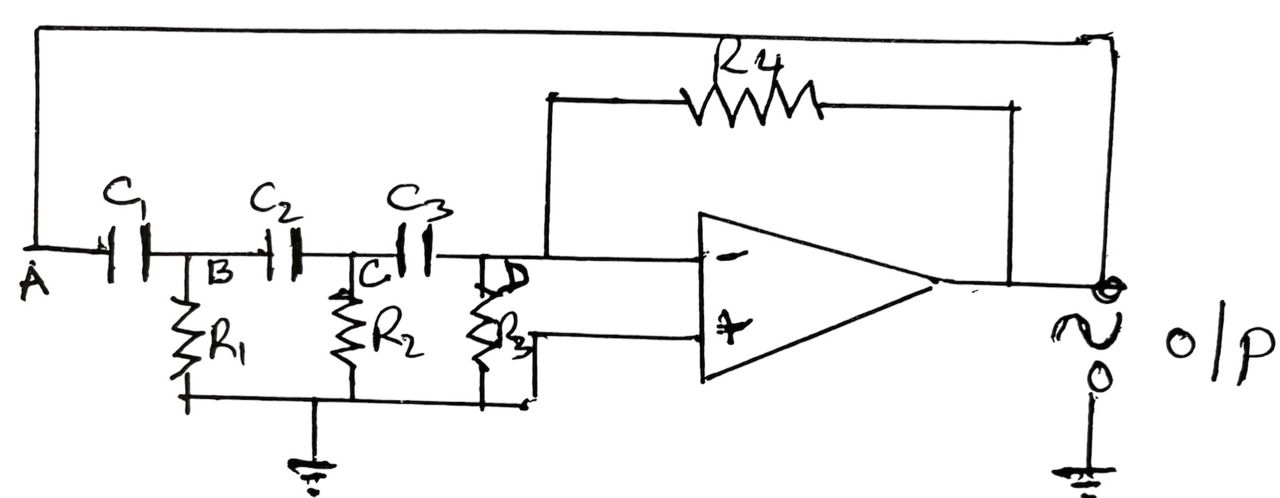
\includegraphics[width=0.5\linewidth]{circuit1_1.jpeg}
            \caption{Basic RC circuit}
            \label{fig:1}
        \end{figure}
        $$ C_1 = C_2 = C_3 = 2.2nF$$
        $$ R_1 = R_2 = R_3 = 10k \Omega$$
        $$ R_4 = 470k \Omega$$
        $$ f = \frac{1}{2 \pi RC \sqrt{6}}$$
        \item Observe the waveform
        \begin{figure}[H]
            \centering
            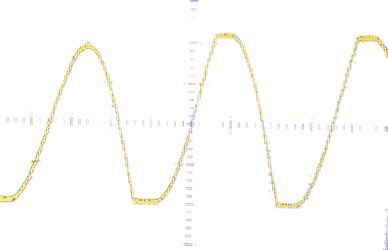
\includegraphics[width=0.5\linewidth]{1.jpeg}
            \caption{RC oscillators}
            \label{fig:enter-label}
        \end{figure}
        \item Compare the wave forms at points ABCD
        \begin{itemize}
            \item at point A
            \begin{figure}[H]
            \centering
            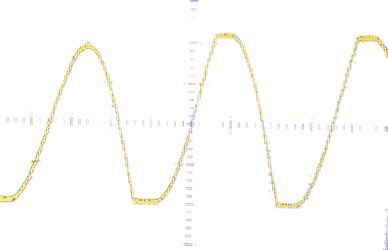
\includegraphics[width=0.5\linewidth]{1.jpeg}
            \caption{wave form at point A}
            \label{fig:enter-label}
        \end{figure}
            \item at point B
            \begin{figure}[H]
                \centering
                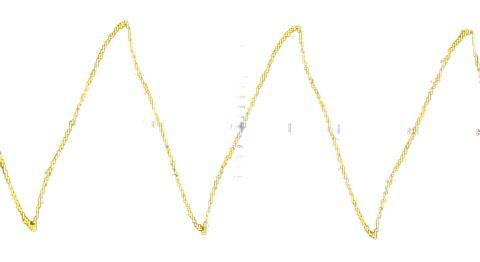
\includegraphics[width=0.5\linewidth]{b.jpeg}
                \caption{Wave form from point B}
                \label{fig:enter-label}
            \end{figure}
    \item at point C
    \begin{figure}[H]
        \centering
        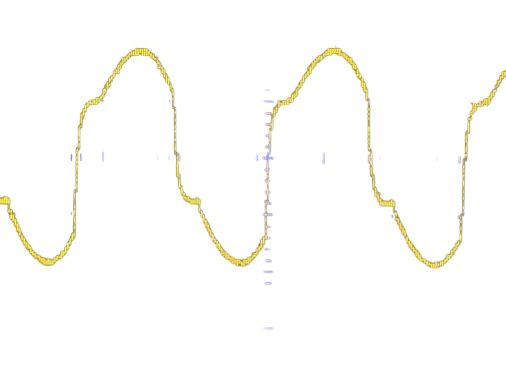
\includegraphics[width=0.5\linewidth]{c.jpeg}
        \caption{wave form from point C}
        \label{fig:enter-label}
    \end{figure}
    \item at point D
    \begin{figure}[H]
        \centering
        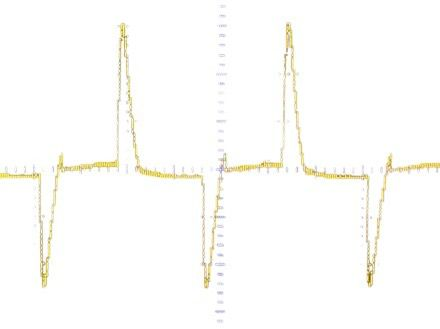
\includegraphics[width=0.5\linewidth]{d.jpeg}
        \caption{wave form from point D}
        \label{fig:enter-label}
    \end{figure}
        \end{itemize}
        \item Compare the frequency output generated with the theoretical frequency using the formula given below\\
        for the practical frequency:\\
        $$ f = 2.878kHz$$
        Theoretical frequency:
        $$ f = \frac{1}{2 \pi RC \sqrt{6}}$$
        $$ f = \frac{1}{2 \pi (10k)(2.2n) \sqrt{6}}$$
        $$ f = 2.95kHz$$
        
    \end{enumerate}

    \subsubsection{Procedure 2 - The wein bridge oscillator}

    \begin{enumerate}
        \item Construct the circuit of the figure:\ref{fig:2} below
        \begin{figure}[H]
            \centering
            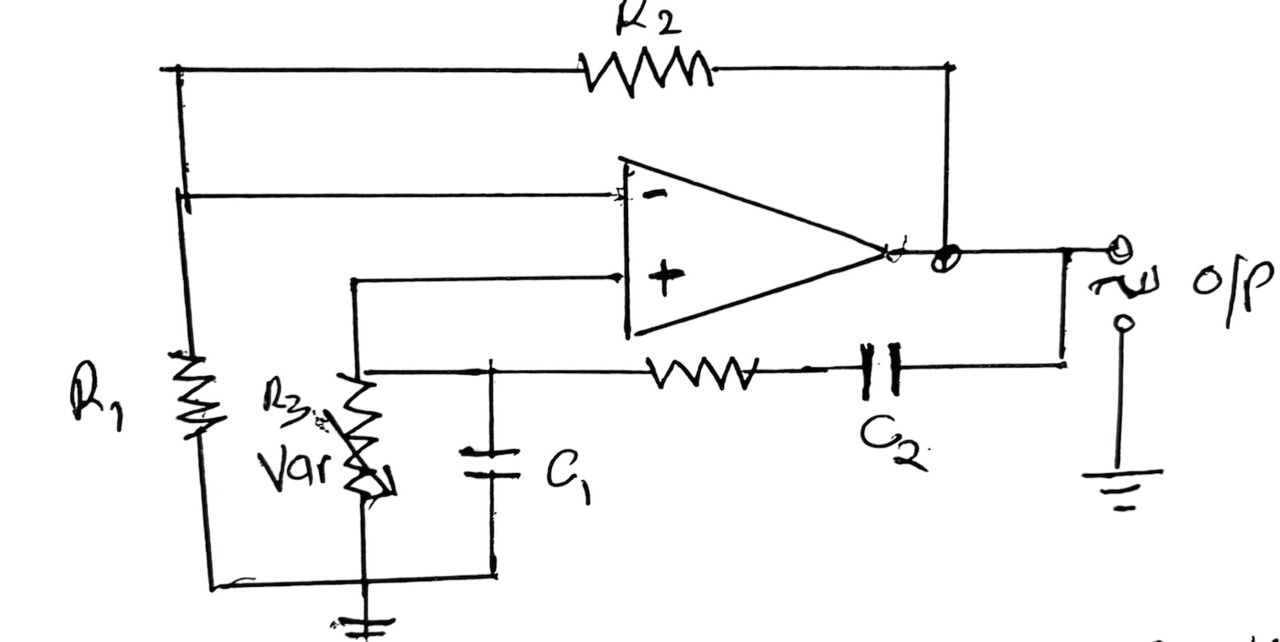
\includegraphics[width=0.5\linewidth]{circuit2_2.jpeg}
            \caption{The wein bridge oscillator}
            \label{fig:2}
        \end{figure}
        Vary $R_3$ for output\\
        $R_1 = 1k \Omega$, $R_2 = nerate plot from picture2.2k \Omega$, $R_3 = 1k \Omega$ variable\\
        $ C_1 = C_2 = 12nF$
        \item Observe the wave form generated
        \begin{figure}[H]
            \centering
            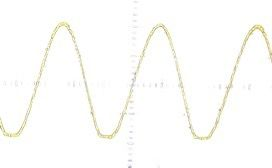
\includegraphics[width=0.5\linewidth]{2.jpeg}
            \caption{wave form for wein bridge oscillator}
            \label{fig:enter-label}
        \end{figure}
        \item Compare the waveform of the phase shift generated and the Wien bridge oscillator
        
        \textbf{\textit{The wave form produced are very similar yet produced with different setups}}
    \end{enumerate}

    \subsubsection{Procedure 3 - The square wave}
    \begin{enumerate}
        \item Construct the circuit of the figure:\ref{fig:3} below
        \begin{figure}[H]
            \centering
            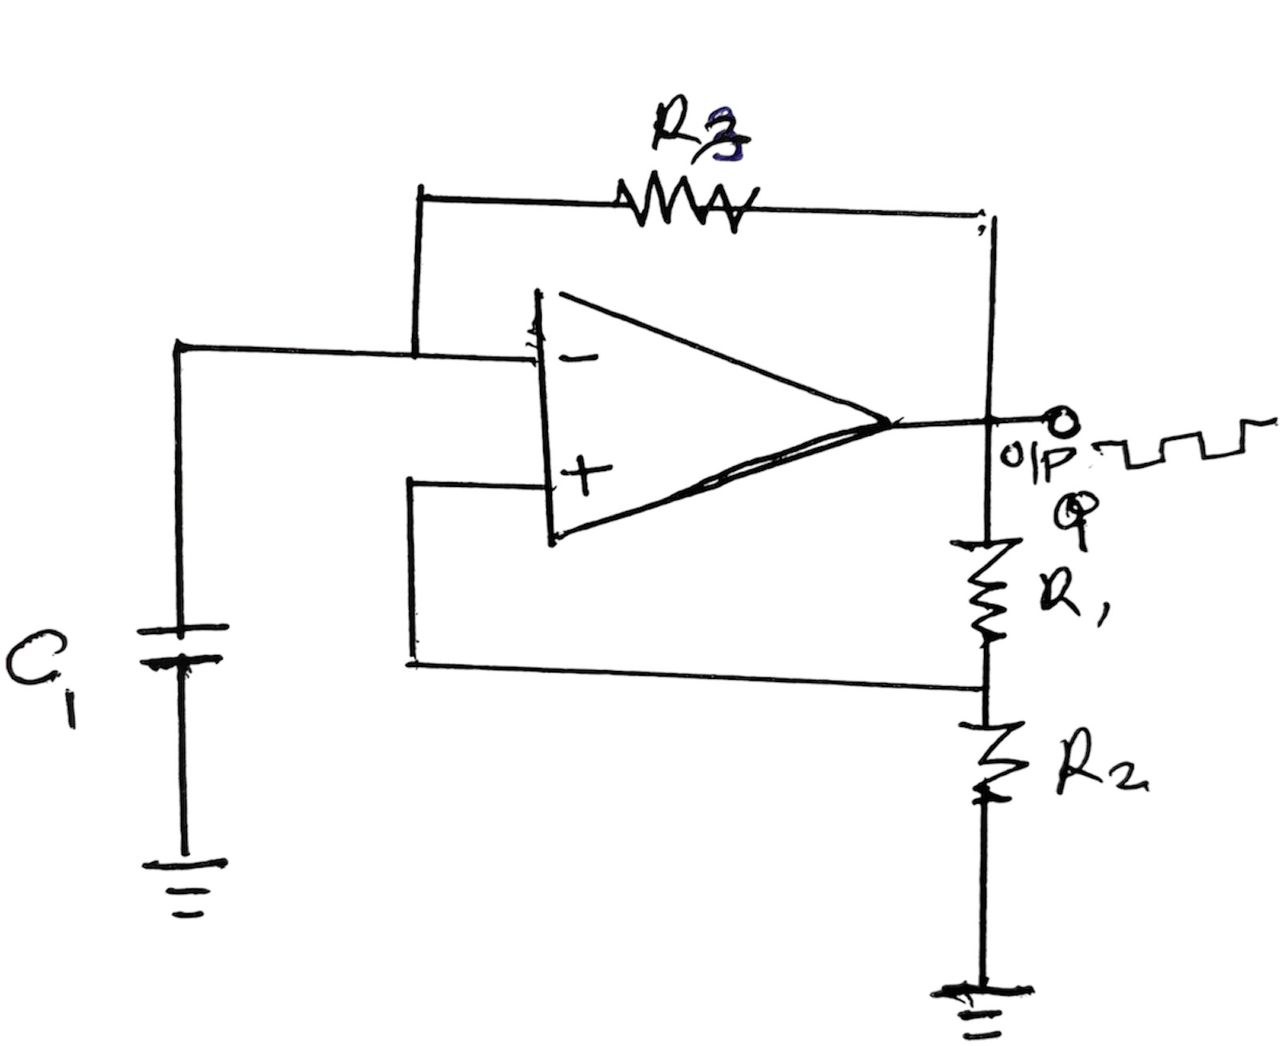
\includegraphics[width=0.5\linewidth]{circuit3_1.jpeg}
            \caption{The square wave}
            \label{fig:3}
        \end{figure}
    \end{enumerate}
    $$ R_1 = R_2 = 10k \Omega$$
    $$ R_3 = 4.7k \Omega$$
    $$ C_1 = 1nF $$
    \subsubsection{Questions}

    What values of the resistor $R_1$ and $C_1$ would make an output of 10OkH?

    \[
    f = \frac{1}{2 \pi RC}
    \]
    Given:
    \[
    R = 10 \, \text{k}\Omega, \quad f = 10 \, \text{kHz}
    \]
    we can rearrange the formula to solve for \( C \):
    \[
    C = \frac{1}{2 \pi R f}
    \]
    Substituting in the values:
    \[
    C = \frac{1}{2 \pi \times 10 \, \text{k}\Omega \times 10 \, \text{kHz}}
    \]
    \[
    C \approx 1.59 \, \text{nF}
    \]
    \[
    \therefore \quad R = 10 \, \text{k}\Omega \quad \text{and} \quad C \approx 1.59 \, \text{nF} \quad \text{will produce} \quad f \approx 10 \, \text{kHz}.
    \]



    \section{Experiment to Demonstrate Amplification with Resistive and Tuned Loads using Class C Amplifiers}
    \subsection{Objectives}
    \begin{enumerate}
        \item Amplification with resistive loads:
        \begin{enumerate}
            \item analysis of bias circuits
            \item inspection of the current wave-form in the load
            \item measurement of the conduction angles as a function of the biasing
        \end{enumerate}
        \item Amplification with tuned loads:
        \begin{enumerate}
            \item calculation of the resonant frequency fo
            \item use as frequency multiplier
        \end{enumerate}
    \end{enumerate}
    \subsection{Instruments}
    \begin{enumerate}
        \item function generator
        \item oscilloscope
        \item multimeter
    \end{enumerate}
    \subsection{Basic Theory}
    Class C amplifiers are designed to operate with the transistor biased below the cutoff point, conducting for less than half of each input signal cycle.
    \begin{figure}[H]
        \centering
        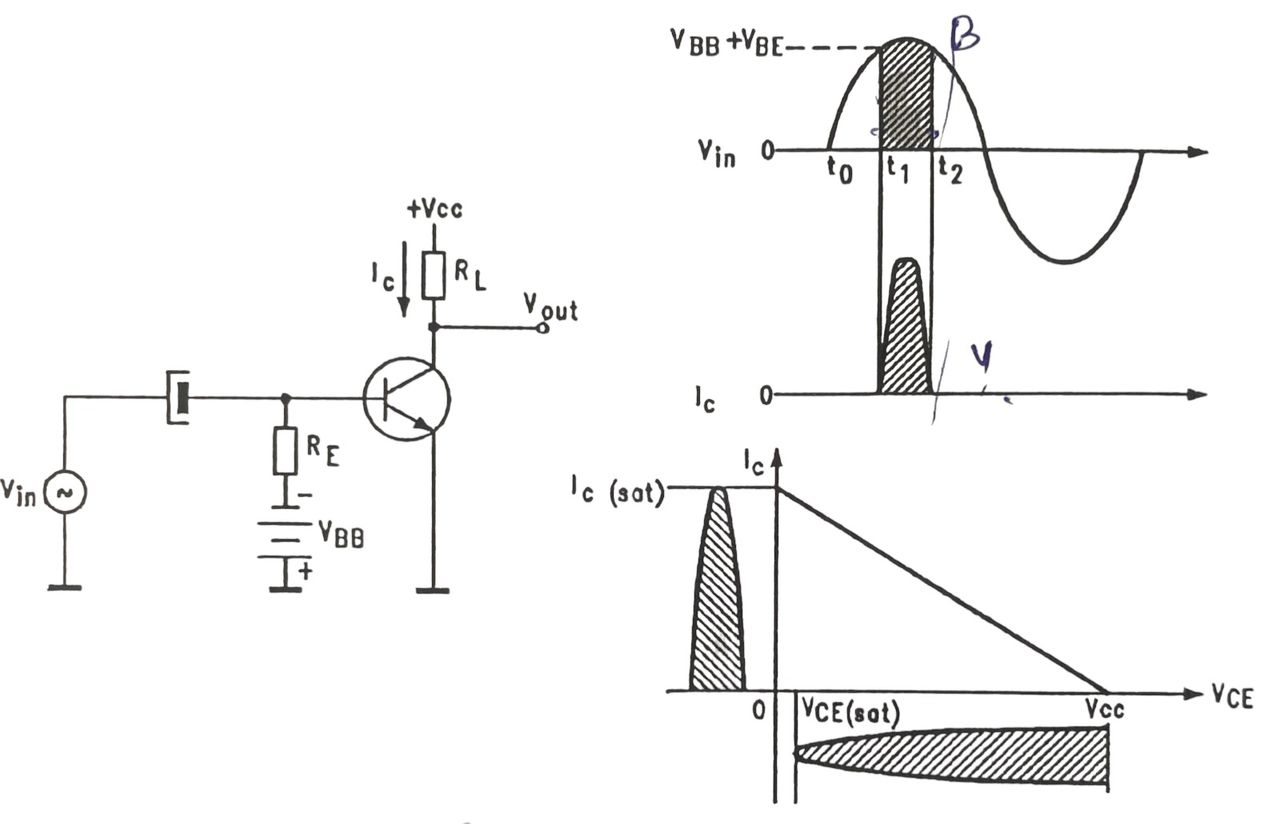
\includegraphics[width=0.5\linewidth]{analogue1_1.jpeg}
        \caption{class C amplifier}
        \label{fig:B32.1}
    \end{figure}
    This mode of operation results in a highly distorted, pulsed output, which requires filtering to achieve a clean output waveform. These amplifiers are inherently non-linear and are unsuitable for applications where low distortion is required.

    Class C amplifiers are highly efficient, often achieving over 80\%, as the transistor only conducts for a small portion of each cycle, minimizing power dissipation. They are typically used with a resonant LC load (inductor-capacitor circuit) tuned to the desired frequency, which filters the pulsed output to create a sinusoidal signal. The resonant frequency \( f \) of the LC circuit is given by:
    \[
    f = \frac{1}{2 \pi \sqrt{LC}}
    \]

    \subsubsection{Applications}
    Class C amplifiers are commonly used in:
    \begin{itemize}
        \item RF Transmitters: Amplifying high-frequency signals for radio and radar systems.
        \item Oscillators: Maintaining oscillations at specific frequencies in communication systems.
        \item FM and AM Transmitters: Amplifying carrier signals for frequency and amplitude modulation.
    \end{itemize}

    \subsubsection{Limitations}
    The limitations of Class C amplifiers include:
    \begin{itemize}
        \item High Distortion: Non-linearity results in significant harmonic distortion.
        \item Limited Frequency Range: Most suitable for high frequencies, requiring large components for low frequencies.
        \item Need for Resonant Loads: Dependence on resonant loads adds complexity to the circuit.
    \end{itemize}

    In summary, Class C amplifiers are ideal for high-efficiency, high-frequency applications where distortion can be tolerated or filtered out.

    \subsubsection{Operation}
    When a sine wave of voltage $v(t) = V_M sin(\omega-t)$, is connected to the input of the amplifier, the current $i(t)$ through the load $R_L$ is different from zero in the conduction range $T = t_2 - t_1$, which corresponds to a conduction angle $\phi = \phi_2 - \phi_1$, where $\phi = \omega T$.
    \\
    \\
    In a class C amplifier the angle $\phi$ is less that 180 degrees, and depends on the transistor bias.
    \\
    \\
    The class C amplifier does not dissipate power in static conditions $I_{CQ} = 0$, while the power dissipated in dynamic conditions depends on the amplitude of the signal $v(t)$ and the conduction angle $\phi$, reducing this angle, the efficiency increases, and can take values approaching 100\%. Actually, we cannot reduce the conduction angle $\phi$ too much, because the overall power decreases too.
    \\
    \\
    The train of pulses constituting the load current $i(t)$ represents a non-sinusoidal, periodic function. The period of this function equals the input signal period. Using a Fourier series, the load current can be represented by an infinite sum of sine waves:
    $$i(t) = I_{CQ} + i_{1}.sin(\omega t) + i_{2}sin(2 \omega t) +...$$
    If a resonant circuit is used as load, tuned at an harmonic of the fundamental, this amplifier can be used as frequency multiplier. Since the amplitude of the higher harmonics falls rapidly as frequency increases, the main amplification will be obtained at the fundamental frequency, i.e. at $f = \frac{\omega}{2 \omega \pi}$.
    \\
    \\
    A class C amplifiers operate at very high efficiency, but is only used to amplify a single frequency. It cannot be used for the linear amplification. For these reasons, it is used with a resonant load to extract the main frequency, or possibly one of its harmonics.
    \subsection{Experiments}
    \subsubsection{Amplifier with resistive load}
    \subsubsection{Procedures}
    \begin{enumerate}
        \item Set Vcc adjustable power supply to 12V.
        \item Insert jumpers $J_1, J_3, J_{10}, J_{11}, J_{15}, J_{17}, J_{26}$, to produce the circuit of figure:\ref{fig:B32.2}
        \begin{figure}[H]
            \centering
            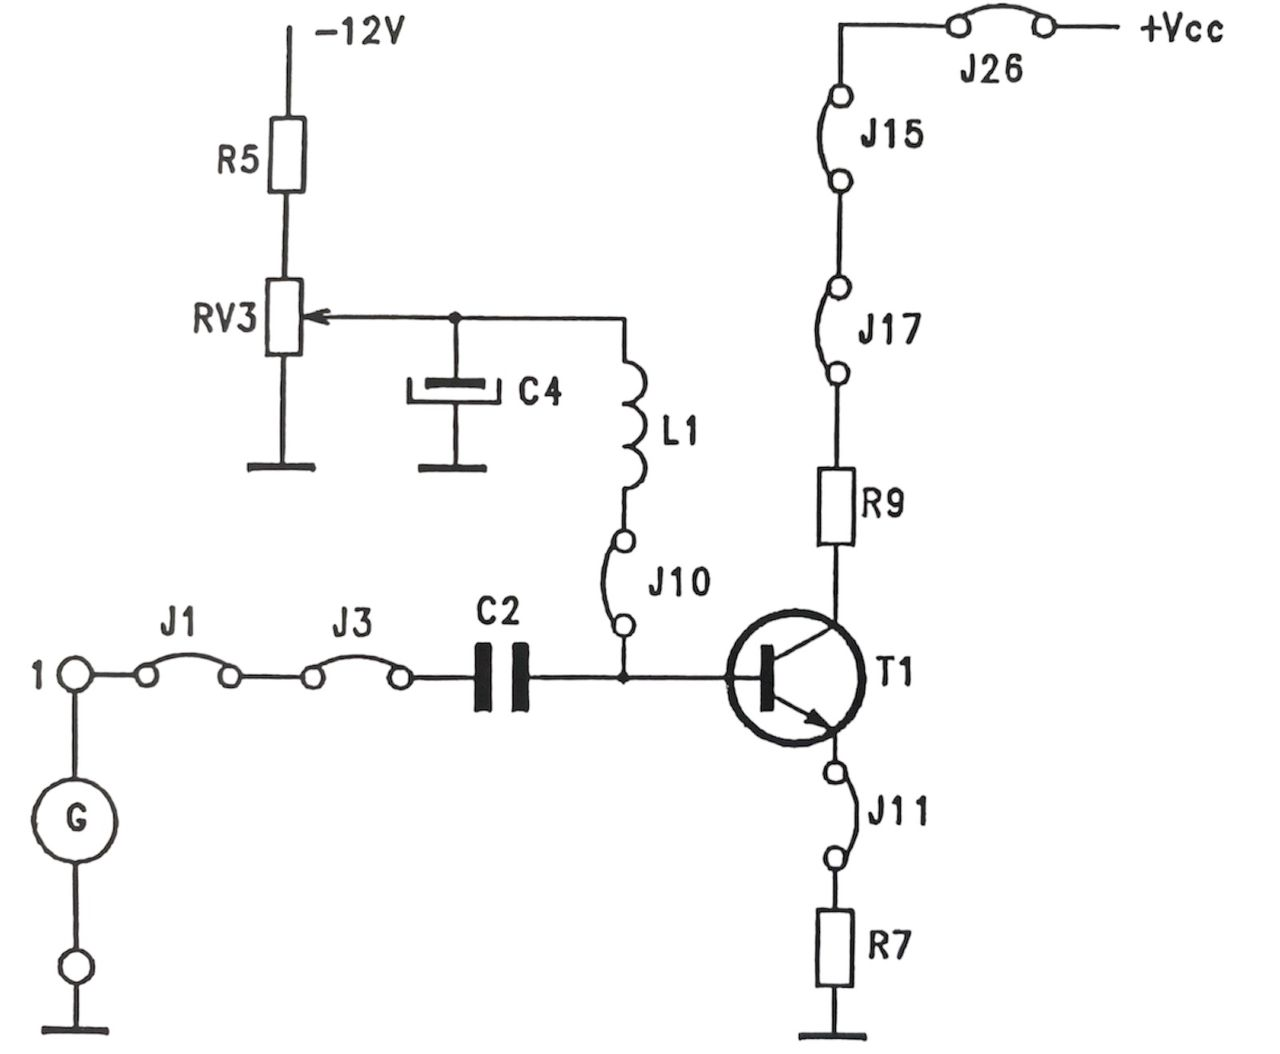
\includegraphics[width=0.5\linewidth]{analogue2_2.jpeg}
            \caption{amplifer with resistive load}
            \label{fig:B32.2}
        \end{figure}
        \item adjust $R_{V3}$, and consider how the bias voltage on the base of transistor $T_1$ varies
        \item connect the function generator at terminals 1 and ground with a sine 20 KHz and 1$V_{pp}$
        \item reduce the frequency of the input signal, and check the resulting signal on base of $T_1$ with oscilloscope
        \item adjust $R_{V3}$ to set the voltage on the base of $T_1$ to 0V
        \item set the sine input signal to 20 kHz
        \item increase the amplitude of the input signal, observing the signal on the collector of $T_1$ and across $R_7$
        \item in particular, analyze the case in which the positive peak of the input voltage, applied across the base of $T_1$, exceeds the threshold 0.6-0.7V of the transistor
        
    \textit{When the input voltage exceeds the transistor threshold voltage it starts conducting generating small voltage pulses ac
    s the resistance $R_7$. As the conduction angle is less smaller than 180 degrees, the amplifier is in class C}

        \item adjust $R_{V3}$ to negatively bias the base of $T_1$ and check the behavior of the voltage across $R_7$
        \item vary $R_{V3}$, and note the conduction angle of the output signal
    \end{enumerate}
    \subsubsection{Questions}
    \begin{enumerate}
        \item How does the amplitude vary with frequency?\\
            \(\square\) it remains constant \\
            \(\square\) it is always zero \\
            \(\square\) it decreases \\
            \(\textcolor{black}{\blacksquare}\) it increases \\
            \(\square\) it has a square-wave behavior\\
            \textit{The inductance $L_1$ separates the bias circuit, consisting of $R_{V3}$ and $R_5$, from the ac input signal. In fact the impedance of an inductance is proportional to frequency, so the higher the frequency, the higher will be reactance of $L_1$, and the better will be the separation. The capacitor $C_4$ is used to short-circuit any remaining signals across $L_1$.}
        \item What happens to the output voltage on $R_7$ as the base bias of Tl is continuously reduced?\\
            \(\square\) the peak amplitudes of the.output signal increase\\
            \(\textcolor{black}{\blacksquare}\) the amplitude of the output peaks decrease\\
            \(\square\) the output signal frequency progressively increases\\
            \(\square\) there is no output change\\
            \(\square\) the phase shift between the input and output signal progressively increases
        \item Comparing the conduction angles obtained with different bias conditions, we can say that:\\
            \(\square\) the conduction angle stays unchanged\\
            \(\square\) the conduction angle increases when the voltage on the base of $T_1$ decreases\\
            \(\textcolor{black}{\blacksquare}\) the conduction angle decreases when the voltage on the base of $T_1$ decreases
    \end{enumerate}
    \subsubsection{Tuned load}
    \subsubsection{Procedures}
    \begin{enumerate}
        \item Remove jumper $J_{17}$ and insert $J_{16}$, to produce the circuit of figure:\ref{fig:B32.3}
        \begin{figure}[H]
            \centering
            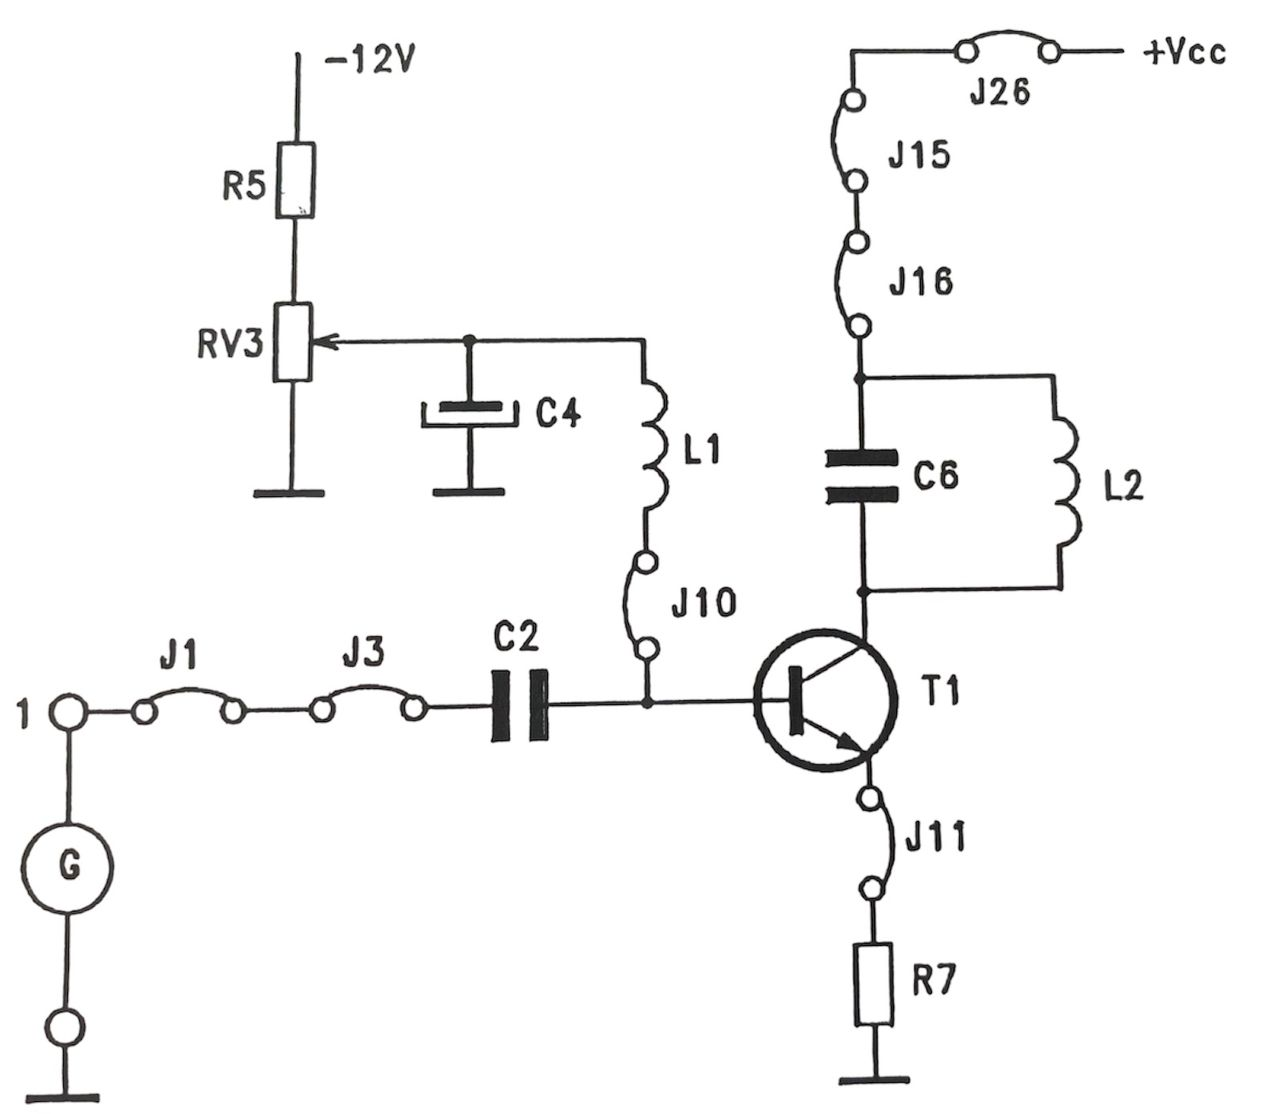
\includegraphics[width=0.5\linewidth]{analogue3_3.jpeg}
            \caption{tuned load}
            \label{fig:B32.3}
        \end{figure}
        \item adjust RV3 to obtain a base bias voltage of 0 V
        \item calculate the resonant frequency of the tuned circuit L2-C6, using the relation $f_o = \frac{1}{2\pi \sqrt{LC}}$, if $L_2 = 4\mu H$ and $C_6 = 680nF$
        \item apply a sine signal of $2V_{pp}$-amplitude and frequency $f_o$ to the input
        \item examine the wave-form of the signal across $R_7$ (proportional to the current through the transistor) and also the signal on the collector
        \item adjust the input frequency to obtain the max. amplitude on the $T_1$ collector ( terminal 3)
        
    \textit{When the frequency of the input signal is equal to the resonant
    frequency of the LC circuit, the output signal amplitude is max and the waveform is nearly distortionless. The amplifier is said to be tuned.}
        \item slowly decrease the input signal frequency, until it is halved, while observing the behavior of the output signal on the $T_1$ collector (terminal 13)
        \item in particular, analyze what happens when the input frequency near $\frac{f_o}{2}$
    \\
    \\
    As the frequency decreases, the amplitude of the output voltage slowly drops if $\frac{f_o}{2}<f<f_o$, the output has a behavior which is not sinusoidal anymore. Continuing to reduce the frequency, the second harmonic of the input signal clearly appears
    \\
    \\
    As the output frequency in this case is double the input signal
    frequency, the circuit can be used as frequency multiplier.
    \end{enumerate}
    \subsubsection{Questions}
    \textbf{Turn switch $S_5$ "ON"}
    \begin{enumerate}
        \item Noting the change in amplifier operation, we can say that:\\
            \(\textcolor{black}{\blacksquare}\) the tuned output circuit has been changed\\
            \(\square\) the base bias has been changed\\
            \(\square\) the resistance $R_7$ has been reduced\\
            \(\square\) the power supply voltage VCC has been decreased\\
            \(\square\) the transistor $T_1$ has been short-circuited between base and collector\\
            
    \textbf{Turn $S_5$ "OFF"}
    \end{enumerate}
    \subsection{Summary Questions}
    \begin{enumerate}
        \item The operation in class Cof an amplifier is characterized by conduction angles:\\
        
    \(\square\) greater than 180 degrees\\
    \(\square\) equal to 180 degrees\\
    \(\textcolor{black}{\blacksquare}\) less than 180 degrees\\
    \(\square\) equal to 360 degrees\\
    \(\square\) equal to 270 degrees

    \item Class C amplification produces a signal distortion which is:\\
    \(\square\) very small\\
    \(\textcolor{black}{\blacksquare}\) very big\\
    \(\square\) similar to the one produced by class A\\
    \(\square\) similar to the one produced by class B\\
    \(\square\) similar to the one produced by class AB

    \item The efficiency of a class C amplifier :\\
    \(\textcolor{black}{\blacksquare}\) depends on the conduction angle and takes very high values on average\\
    \(\square\) is always very low\\
    \(\square\) is always equal to 1\\
    \(\square\) is close to 25\% \\
    \(\square\) is equal to 50\% \\

    \item A tuned load in an amplifiers operating in class C can be used toproduce:\\

    \(\square\) a frequency divider\\
    \(\textcolor{black}{\blacksquare}\) a frequency multiplier\\
    \(\square\) a half-wave rectifier\\
    \(\square\) a voltage stabilizer\\
    \(\square\) a current limiter
    \end{enumerate}

    \section{Errors}

    Errors refer to the deviations or differences between the measured value and the true value of a quantity.

    Errors can arise due to limitations in the equipment, environmental factors, the method of measurement, or human factors, and they impact the accuracy and reliability of results. 
    \subsection{Sources of Errors}
    \begin{enumerate}
        \item Oscillators: Potential sources of errors include:
        \begin{enumerate}
            \item Increased resistance within the connecting probes/wires
            \item Power fluctuations within some components
            \item Loose connections
        \end{enumerate}
        \item Class C Amplifiers: Potential sources of errors include:
        \begin{enumerate}
            \item biasing issues
            \item component tolerances
            \item temperature effects
            \item mismatched load
            \item loose connections
        \end{enumerate}
    \end{enumerate}
    \subsection{Error minimization}
    \subsection{Error Minimization}

    To improve the accuracy of the experimental results and reduce errors, specific steps can be taken in circuit design and setup. The following are recommended practices for minimizing errors in different components used in the experiment:

    \begin{enumerate}
        \item \textbf{Oscillators}
        \begin{itemize}
            \item \textbf{Limit Resistive Elements:} Reducing the number of resistive elements in the circuit helps minimize potential sources of resistance-based error and improves signal stability.
            \item \textbf{Ensure Tight Connections:} Loose connections can cause fluctuating voltages and other errors in the oscillator circuit. Ensuring all connections are secure reduces noise and improves the reliability of the signal.
        \end{itemize}
        
        \item \textbf{Class C Amplifiers}
        \begin{itemize}
            \item \textbf{Calibrate Devices Accurately:} Regular calibration of measuring devices and components within the Class C amplifier circuit is essential to minimize calibration-related errors, which can lead to inaccuracies in gain and frequency response.
        \end{itemize}
    \end{enumerate}

    \section{Conclusion}

    By constructing and analyzing these circuits, we gained hands-on experience with signal generation and amplification. The experiments provided insights into the importance of minimizing errors through careful circuit design and calibration.

    Overall, this practical approach enhanced our understanding of analouge electronics, reinforcing theoretical knowledge and highlighting the applications and limitations of oscillators and Class C amplifiers in real-world scenarios.

    \nocite{*}
    \bibliographystyle{ieeetr}
    \bibliography{ref}
\end{document}
